\documentclass[journal]{vgtc}                % final (journal style)

\usepackage{indentfirst} %MCW added

%% These few lines make a distinction between latex and pdflatex calls and they
%% bring in essential packages for graphics and font handling.
%% Note that due to the \DeclareGraphicsExtensions{} call it is no longer necessary
%% to provide the the path and extension of a graphics file:
%% 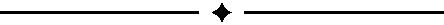
\includegraphics{diamondrule} is completely sufficient.
%%
\ifpdf%                                % if we use pdflatex
  \pdfoutput=1\relax                   % create PDFs from pdfLaTeX
  \pdfcompresslevel=9                  % PDF Compression
  \pdfoptionpdfminorversion=7          % create PDF 1.7
  \ExecuteOptions{pdftex}
  \usepackage{graphicx}                % allow us to embed graphics files
  \DeclareGraphicsExtensions{.pdf,.png,.jpg,.jpeg} % for pdflatex we expect .pdf, .png, or .jpg files
\else%                                 % else we use pure latex
  \ExecuteOptions{dvips}
  \usepackage{graphicx}                % allow us to embed graphics files
  \DeclareGraphicsExtensions{.eps}     % for pure latex we expect eps files
\fi%

\usepackage{microtype}                 % use micro-typography (slightly more compact, better to read)
\PassOptionsToPackage{warn}{textcomp}  % to address font issues with \textrightarrow
\usepackage{textcomp}                  % use better special symbols
\usepackage{mathptmx}                  % use matching math font
\usepackage{times}                     % we use Times as the main font
\usepackage{caption}		% caption for table
\renewcommand*\ttdefault{txtt}         % a nicer typewriter font
\usepackage{cite}                      % needed to automatically sort the references

%% Paper title.
\title{World Leader Interactions on Social Media (Twitter) \\
CS 725/825, Fall 2017}

%% This is how authors are specified in the journal style

%% indicate IEEE Member or Student Member in form indicated below
\author{Grant Atkins\\
Department of Computer Science\\
Old Dominion University\\
Norfolk, VA 23529\\
gatkins@cs.odu.edu
}
\authorfooter{
}

%other entries to be set up for journal
\shortauthortitle{Biv \MakeLowercase{\textit{et al.}}: Global Illumination for Fun and Profit}
%\shortauthortitle{Firstauthor \MakeLowercase{\textit{et al.}}: Paper Title}

%% Abstract section.
\abstract{
Social media has become a platform that world leaders have 
begun to use to express their voice to the public.  Twitter in particular,
is interacted with frequently with data open to users publicly which allows
for developers to take this data and visualize it for each user. Many 
visualizations have been created using Twitter data before and Twitter
itself offers an analytics dashboard for users to explore. 
This however is limited as it represents single user not Twitter lists.
To alleviate this problem, an interactive dashboard was built to visualize ways
a twitter lists data can be used and represented in different ways. 
For this visualization we used the World Leaders list on twitter, with the addition 
of a few world leaders not on the list, to derive information and visualize shared information 
among these users. 
The goal of this visualization is to show 
shared term usage among world leaders, see which times tweets are more likely
to be sent out, the sentiment of the users, and the decay of data allocated
in a static decreasing time interval.
} % end of abstract

%% Uncomment below to include a teaser figure.
\teaser{
  \centering
  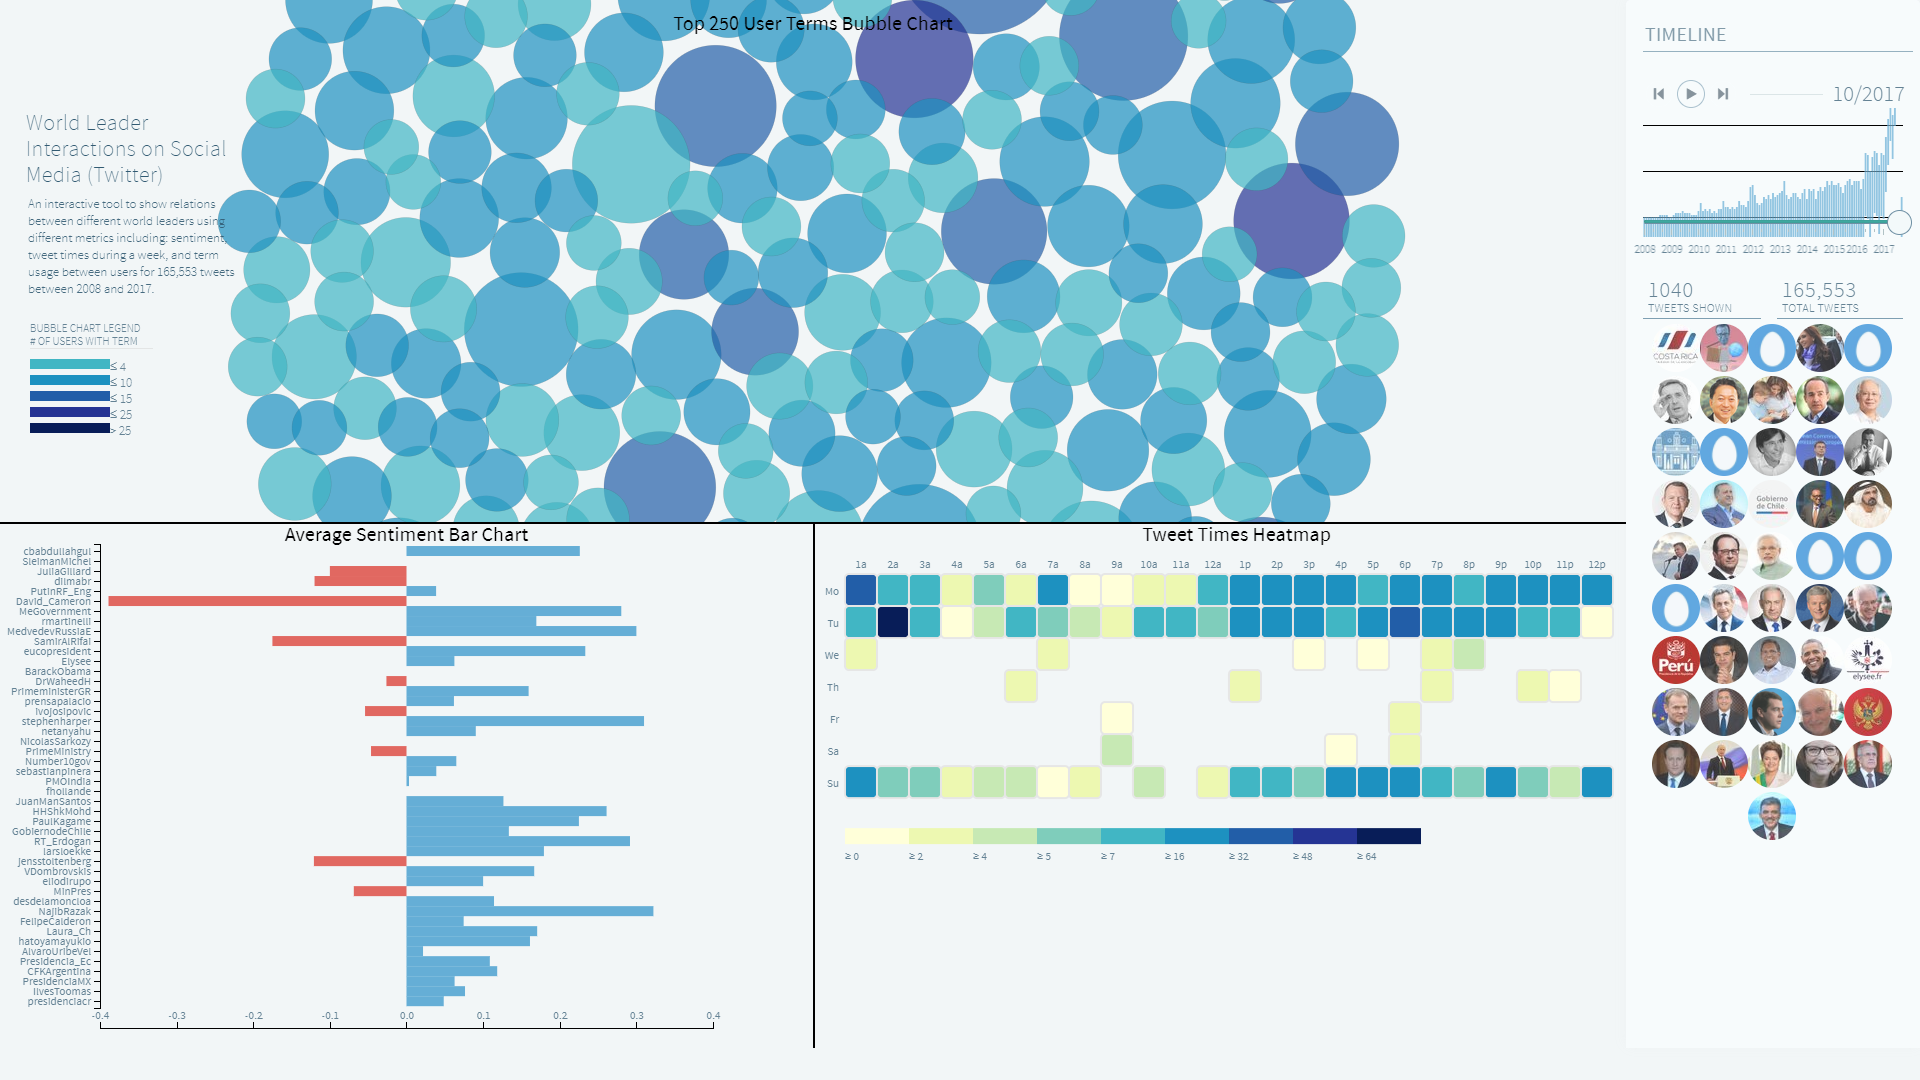
\includegraphics[width=\linewidth]{imgs/world-leader-vis.PNG}
  \caption{World Leader Interactions on Social Media (Twitter) Visualization Web page. Includes four visualizations: average sentiment bar chart, tweet times heatmap, tweet counts bar chart, and top 250 terms in tweets bubble chart.}
	\label{fig:teaser}
}

%% Uncomment below to disable the manuscript note
\renewcommand{\manuscriptnotetxt}{}

%% Copyright space is enabled by default as required by guidelines.
%% It is disabled by the 'review' option or via the following command:
 \nocopyrightspace

\vgtcinsertpkg

%%%%%%%%%%%%%%%%%%%%%%%%%%%%%%%%%%%%%%%%%%%%%%%%%%%%%%%%%%%%%%%%
%%%%%%%%%%%%%%%%%%%%%% START OF THE PAPER %%%%%%%%%%%%%%%%%%%%%%
%%%%%%%%%%%%%%%%%%%%%%%%%%%%%%%%%%%%%%%%%%%%%%%%%%%%%%%%%%%%%%%%%

\begin{document}

%% The ``\maketitle'' command must be the first command after the
%% ``\begin{document}'' command. It prepares and prints the title block.

%% the only exception to this rule is the \firstsection command
\firstsection{Introduction}

\maketitle

Social media outlets have increasingly become a data source for developers to parse, interpret, and visualize.
Most of these outlets allow for groups or communities to be created that contain groups of users on their respective platforms.
Each user on these platforms has data collected from them including: messages, posts, profile images, timestamps, and much more.
The data features just listed are just a small example, but when you pool multiple users together it starts to form large aggregated sets of data representing groups.
Although studying single users is interesting on its own, its become more common to group particular users together and then visualize their data together.

Platforms such as Twitter, Facebook, WhatsApp, and others, have these groups and provide APIs to collect data from individual users as well as groups.
Twitter in particular is very simple and easy to get access to as it allows access to every public user's data for a maximum of 3200 tweets retrieved from a user's timeline.
With the data provided by Twitter I decided to find out what sort of visualizations I could create based on aggregated data of multiple users attempting to find association between users and user actions.

For this visualization I took user data from a list located on Twitter named World Leaders, which currently contains a list of 65 world leaders located globally, with the addition of the current United States president Donald J. Trump and Russian Federation president Vladimir Putin.
With the collection of this data there are many problems with separating, cleaning, translating, and then ultimately combining the aggregated data together that is discussed later in section \ref{data-ref}.
Users in this data may be out dated, in the sense that they no longer use or update their profile on Twitter.
To compensate for this I set intervals of a period of one month for every month that had data from what I retrieved from each user on Twitter.

The resulting visualization dashboard allows for a user to explore the World Leader data extracted from Twitter seeing the top term usages for each month from 04/2008 to early 10/2017.
From this data users will be able to see overlapping details between users and be able to derive meaning for the type of data found on each user but more accurately an overall summarization around the group for each time interval.

\section{Related Work}

A work that was largely influential on this idea and the choice of choosing world data was inspired by a radial dendrogram visualization named FTA-VIS \cite{fta-vis}.
This visualization took data on worldwide trade agreements and showed relations between countries that had this trade agreement.
The idea of neighboring countries relating to each directly influenced the choice of showing term overlap among users.
I also was influenced by the design choices for their visualization and actually used a portion of the HTML/CSS to create a pleasant dashboard.

Another work that was created recently relating to categorizing text of users for showing political sides is a project called Scattertext \cite{kessler2017scattertext}.
This work takes document corpuses and attempts to categorize text based on a users uses of the terms.
This relates to our work mainly due to the fact that a major stepping stone was to figure how to relate users in a categorical way or in a generic term usage way.
Unfortunately our data was too sparse to include this library but it is a good reference for categorical text data visualizations.

Although the afore mentioned projects were the only projects that directly influenced this visualization dashboard, there have been numerous other visualizations applied to Twitter data.
The Twitter platform employs data visualization experts and has its own visualization projects available to the public which are all inspiring when attempting to visualize Social Media data.
Most of the time these visualizations are centered around a topic however and then the visualizations are based on that topic.

\begin{figure}[tb]
 \centering % avoid the use of \begin{center}...\end{center} and use \centering instead (more compact)
 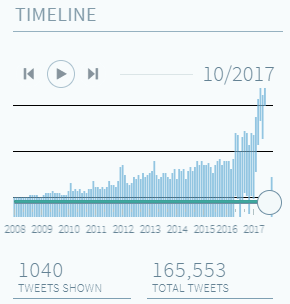
\includegraphics[height=7cm,width=\columnwidth, keepaspectratio]{imgs/timeline.png}
 \caption{Static timeline bar chart showing tweet counts over time for a given collection. This highlights that there is decrease in overall number of tweets going back in time as we don't have access to them given a limit specified by twitter.}
 \label{fig:statbar}
\end{figure}

\section {Data} \label{data-ref}
Describe the data used in your visualization, including citations and links to where it was obtained

As mentioned before, the data used for this visualization dashboard is a list of World Leaders obtained from Twitter \cite{twit-worldlist} found here: \url{https://twitter.com/verified/lists/world-leaders/members?lang=en}.
This list contained 65 members at the time of data collection on October 02, 2017.
Twitter allows for developers to extract tweets from a public twitter user's timeline feed, up to a maximum of 3200 tweets per user.
This 3200 maximum becomes a caveat when trying to effectively visualize the tweet times over a interval of time.
Some of the users in this list did not have 3200 tweets, some reached it within two years, others spread out over a time period of 5 years making it highly variable.
This intrinsically shown in Figure \ref{fig:statbar}, which is a static bar chart on the number of tweets over a time period of 2008 to the collection date of 10/2017. 
A majority of tweets are close to the current time but decline as we go further back in time.

The twitter API offers a large amount of data for each user from which I extracted all that was provided but we only used the following data points in our visualization:

\begin{itemize}
  \item User ID
  \item Tweet ID
  \item User creation date
  \item User screen name
  \item User name
  \item User profile image URL
  \item Tweet text
  \item Tweet timestamps
\end{itemize}

From this data we could extract numerous information and features already.
At the beginning of this project there was the idea of collecting tweet location, user locations, and tweets directed at other users.
However, it became clear quickly that there were very few data points that actually mentioned a location or that a tweet was directed at a user.
I found that of all the tweets that mentioned another user there were only 18. 
It was also found that 15 of these 18 tweets were actually directed at a single user, President Donald J. Trump.
This showed that wasn't enough information to justify creating a visualization that represents an entire list of users.

With 67 users total, I also had to clean the tweets provided.
When merging text data its often required that all of the text be in a single language.
With my dataset being a list of ``World'' leaders, at least 30 of the users did not speak the desired language, English.
To solve this problem I transformed all of the non-english tweets to english using the Google Translate API: \url{https://translate.google.com}.
Timestamps also had to be considered in this visualization as each world leader could be in a different time zone.
Fortunately Twitter automatically gives back data timestamps for a developer's local timezone, therefore all the tweet times are based on Eastern Standard Time. 

Finally after converting everything to english I discovered the world leader list on Twitter actually contained duplicate users.
Some of the world leaders were bi-lingual and created two separate accounts for each language.
For this I simply removed the user accounts that were non english duplicates.
In the end I had 64 unique users with 165,799 tweets.

Then finally I had to transform the data into a format that could be supplied to a web browser that could be interpreted visualized easily.
When this was completed it was interestingly noted that there were 246 tweets at exactly the same timestamps of another tweet.
This was easily solved by simply adding tweets to the same timestamp. 

Each visualization required a different format of data.
For the tweet times heatmap, the required data points were times of the tweets which was broken up into by day and hour of tweet.
The average sentiment bar chart required that the text have some sort of sentiment value applied to all the tweets for a given user for a given time.
To get the sentiment values for each tweets for a given user I used a python library called Textblob \cite{tblob} which provided access to a part of speech (POS) tagger which gave a sentence a polarity value of positive, negative, or zero. Positive represents positive sentiment, negative represents negative sentiment, and zero represented a neutral statement.
I averaged the sentiment values of all the tweets for the user for the given month which is the resulting value for the sentiment bar graph.
For the bubble plot, I took the tweets for all the users for a given month and found the top 250 terms, terms that had the highest repetition in the corpus, and found which users referenced this term at least once.
Finally for the side bar there is a static bar plot that contains months in each year and the number of tweets each year has.
Below the static bar chart there is a section containing all the user profile images linking to their profile images as shown in Figure \ref{fig:users}.
The repeating eggs in this Figure show that the profile image links provided at the time of data collection have been changed from what they originally were.

\begin{figure}[tb]
 \centering % avoid the use of \begin{center}...\end{center} and use \centering instead (more compact)
 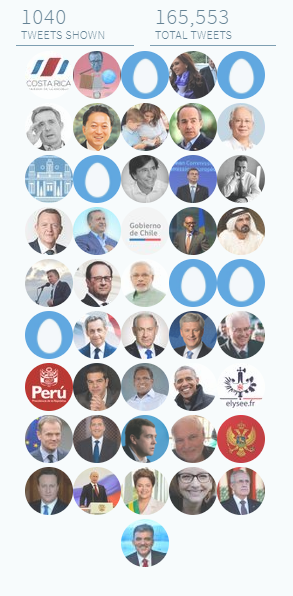
\includegraphics[height=10cm,width=\columnwidth, keepaspectratio]{imgs/twitter-users.png}
 \caption{A snapshot of the user profile images and tweet counts for October 2017 }
 \label{fig:users}
\end{figure}

\section{Visualization}
%Describe the main features and idioms used in your visualization

The visualizations in this dashboard consist of four different visualizations: tweet times heatmap, positive and negative sentiment bar chart, tweet counts and tweet month static bar chart. 
The user interactions on these visualizations is mostly centered around mouseover events triggered by a user and also explicit feedback events for selecting which month of the year a user wants to see.
The sidebar, on the right side shown in Figure \ref{fig:teaser}, contains the static bar chart but also the main interactive parts of this application.
One the goals was to allow users to see tweets over a time periods, in this case months in each year, therefore there is a slider below the tweet counts bar chart that allows user to select it and then slide to the desired dates. 
There is also a previous, play, and next buttons much like a video player as shown in Figure \ref{fig:statbar}.
If a user wants to step to a month before the current one the user presses the previous arrow, which is the reverse if a user presses the next arrow.
There is also built in automation of counting down the date by pressing the play button, which then refreshes the data every three seconds for the previous month of the current month, essentially stepping left every three seconds.
Every time the month is changed in the dashboard all, except the sidebar tweet count bar chart, are updated with the current month data.

The heatmap, as shown in Figure \ref{fig:hmap}, uses tweet time data and plots in a 7x24 grid representing days of the week and an hour in a day.
Users may hover over a piece of the grid that has a color and it show the number of tweets for that given time.
This visualization is meant to be fairly dense with a blocks spatial positions parallel to other blocks showing that each hour and day are one after another, much like a calendar.

The sentiment bar chart is straightforward in the sense it has three options of classification: negative, positive, or neutral.
It has binary colors of red and blue indicating negative and positive sentiment respectively.
When a user hovers on the bar they see the POS sentiment value assigned as stated in section \ref{data-ref}.

The bubble plot was revised a few times, but the resulting visualization was appealing.
Each bubble represents one of the top 250 words found repeatedly in a month.
The size of the bubble is dependent on the number of times the word was found.
The color of the bubble is based on the number of users who used that word in a tweet for the given month.
This bubble plot is different from a scatterplot in a sense that it doesn't plot the spatial position.
This is due to the fact there isn't a third attribute that could be used for spatial position.
If a user hovers on one of the bubbles they can see the the word, the word count, and the profile image of the users who used that word.

\begin{figure}[tb]
 \centering % avoid the use of \begin{center}...\end{center} and use \centering instead (more compact)
 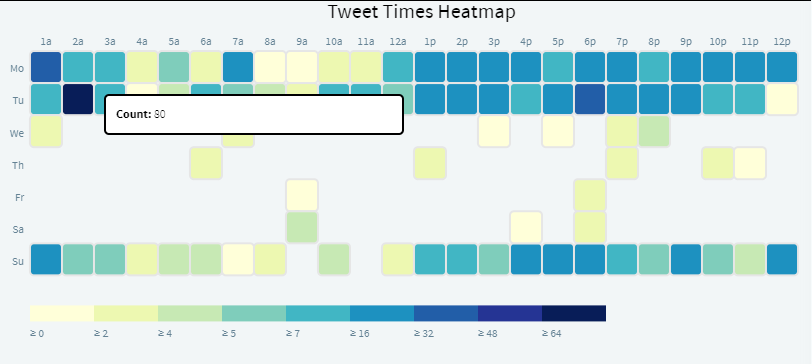
\includegraphics[height=7cm,width=\columnwidth, keepaspectratio]{imgs/heatmap.png}
 \caption{Heatmap of tweet times for a given day and hour of the day for October 2017. The color encoding is that light colors display a lower amount of tweets occurred at the time on the heatmap. As the colors get dark on the heatmap this shows the tweet density around that time. }
 \label{fig:hmap}
\end{figure}

\begin{figure}[tb]
 \centering % avoid the use of \begin{center}...\end{center} and use \centering instead (more compact)
 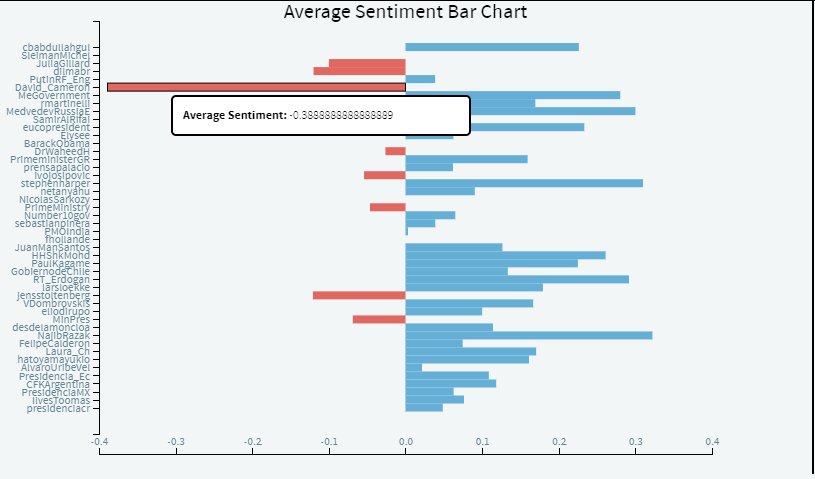
\includegraphics[height=7cm,width=\columnwidth, keepaspectratio]{imgs/sentiment.png}
 \caption{Heatmap of tweet times for a given day and hour of the day for October 2017. The color encoding is that light colors display a lower amount of tweets occurred at the time on the heatmap. As the colors get dark on the heatmap this shows the tweet density around that time. }
 \label{fig:sent}
\end{figure}

\begin{figure*}
 \centering
 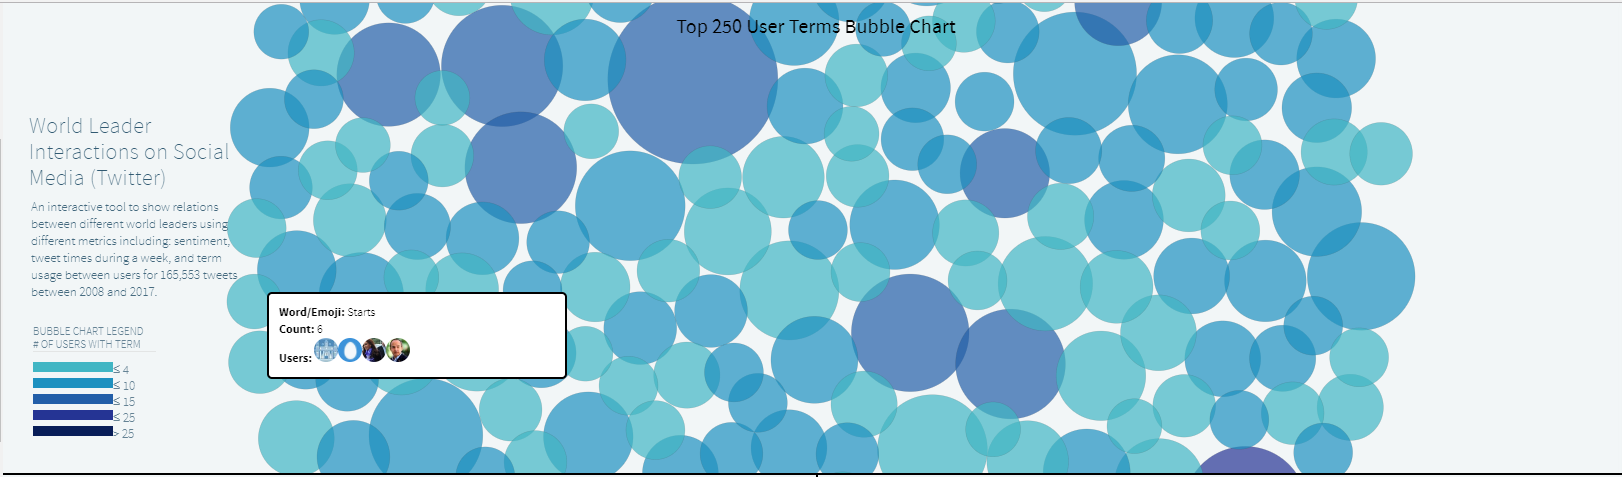
\includegraphics[height=6cm,width=0.8\linewidth]{imgs/bubble.png}
 \caption{Bubble plot with two quantitative values: color and size.}
 \label{fig:sample-2}
\end{figure*}

\subsection{Design Decisions}
%This may be a subsection of the Visualization section.
%Discuss any design decisions made, including those made at the data/task abstraction level and the visual encoding/interaction idiom level (as done in Chapter 4).

The design decisions for this visualization dashboard for mapping color mainly focus on luminance.
The bubble plot and the heatmap take advantage of luminance by showing that the data is ordered based on counts.
In the bubble plot the color gets darker for approximately every five users who share the same term.
This color mapping is shared with the heatmap.
The last 5 shades of the heatmap are the same colors as the five for the bubble plot.

The reason the bubble chart was chosen as the visualization for this dashboard is because it was relatively simple to use two dimensional data on the chart: size and color. 
Color represents the amount of users shared a term while size represents the actual number of times that term is repeated for that month.
These two quantities could have easily be swapped to represent the data for this visualization.
I considered doing k-means clustering and showing how these cluster together, but this data was without topics.
When retrieving this data it wasn't based on a specific event or a specific user but rather a group and the goal is to discover overlap among users. 
In k-means, user has to provide the number of clusters to cluster on which is usually based on a chosen topic.
Since there was not set topic this type of visualization was not chosen for the dashboard.

There were other times I considered redesigning the sentiment bar plot.
There are 3 classifications: positive, negative, and neutral.
A stacked bar plot could have also worked.
What is shown through the months though is that there are hardly any negative or neutral users over time, they're almost all positive.
Therefore, it was chosen to simply have binary colors for positive and negative bars showing that they go in different directions for different values.

%\begin{figure*}
% \centering
% 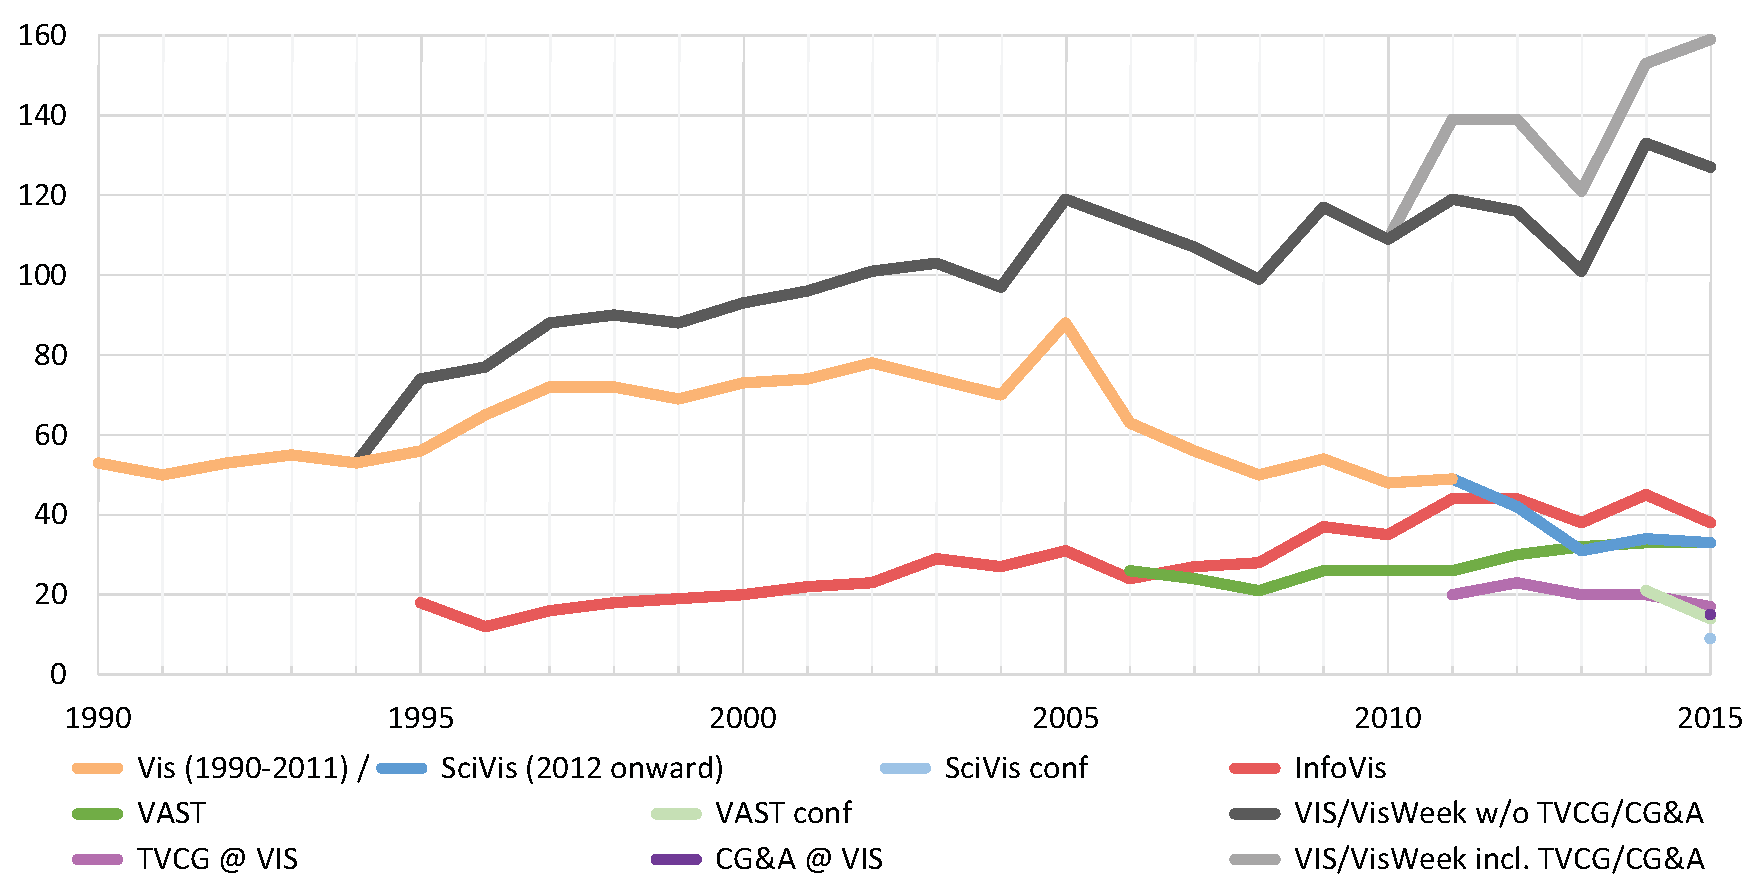
\includegraphics[width=0.8\linewidth]{paper-count-w-2015-new}
% \caption{Showing a single-column image over the two-column text.}
% \label{fig:sample-2}
%\end{figure*}

\section{Analysis}
%Analyze your system using the what/why/how framework, including creating a table as in Chapter 7. If you use multiple idioms, you may need to include multiple tables.
%There are some nice examples of how to frame this in Chapter 15.  For each of the visualization tools in that chapter, there's a table that describes things like "what: data", "what: derived", "why: tasks", "how: encode".

The following tables are the analysis of the what/why/how framework for each visualization. 
The bubble chart, average sentiment bar chart, tweet times heatmap, and tweet counts bar chart are shown in Figures \ref{tab:bb}, \ref{tab:as}, \ref{tab:hm}, and \ref{tab:st} respectively.

\begin{center}
    \captionof{table}{Bubble chart what/why/how framework} \label{tab:bb} 
    \begin{tabular}{ | l | p{4cm} |}
    \hline
    System   & Bubble chart \\ \hline
    What: Data   &  Three quantitative value attributes \\ \hline
    Why: Tasks  & Find trends, outliers, distribution, correlation; locate clusters. \\ \hline
    How: Encode   & Express values with size, color, and unigram. \\ \hline
    Scale  & Items: hundreds. \\ \hline
    \end{tabular}
\end{center}

\begin{center}
    \captionof{table}{Average sentiment bar chart what/why/how framework} \label{tab:as} 
    \begin{tabular}{ | l | p{4cm} |}
    \hline
    System   & Bar chart \\ \hline
    What: Data   & Table: one quantitative value attribute, two categorical key attributes. \\ \hline
    Why: Tasks  & Lookup and compare values. \\ \hline
    How: Encode   & Line marks, express value attribute with aligned horizontal position, separate key attribute with vertical position. \\ \hline
    Scale & Key attribute: 1 - 65 levels \\ \hline
    \end{tabular}
\end{center}

\begin{center}
    \captionof{table}{Tweet times heatmap what/why/how framework} \label{tab:hm} 
    \begin{tabular}{ | l | p{4cm} |}
    \hline
    System   & Heatmap \\ \hline
    What: Data   & Table: two categorical key attributes (day, hour), one quantitative value attribute (number of times hour repeated). \\ \hline
    What: Derived   & Times that cluster well for tweet activity \\ \hline
    Why: Tasks  & Find clusters, outliers; summarize. \\ \hline
    How: Encode   & 2D matrix alignment of area marks \\ \hline
    Scale  & Items: one million. Categorical attribute levels: 7 x 24 (168). Quantitative attribute levels: 3 - 11. \\ \hline
    \end{tabular}
\end{center}

\begin{center}
    \captionof{table}{Tweet counts bar chart what/why/how framework} \label{tab:st} 
    \begin{tabular}{ | l | p{4cm} |}
    \hline
    System   & Bar chart \\ \hline
    What: Data   & Table: one quantitative value attribute, one categorical key attributes. \\ \hline
    Why: Tasks  & Lookup and compare values. \\ \hline
    How: Encode   & Line marks, express value attribute with aligned vertical position, separate key attribute with horizontal position. \\ \hline
    Scale & Key attribute: dozens to hundreds of levels. \\ \hline
    \end{tabular}
\end{center}


\section{Insights or Case Study}
%Show a concrete example of how the visualization addresses the abstract tasks proposed

Two concrete examples of how the visualization addresses the abstract tasks are screenshots taken from four consecutive months for the heamap and sentiment bar charts.
We can see from Figure \ref{fig:all-pos} that an overwhelmingly majority of World Leaders are shown to have positive sentiment each month on public social media platforms such as Twitter. 
There may be times when users show negative sentiment but in this group of World Leaders there was never a month where negative sentiment outweighed positive sentiment.

The heatmap also shows that at certain times of the day, and also certain times of the week, tweets are more likely to go out for World Leaders.
Figure \ref{fig:hmap-dense}, shows four separate heatmap entries for monday through friday from 2pm to 8pm.
This shows that there is density around the times 4pm to 7pm for any given weekday.
This might show that our World Leaders enjoy their weekend get aways and make the public happy on weekdays, but going that far is speculating too much.

\begin{figure}[tb]
 \centering % avoid the use of \begin{center}...\end{center} and use \centering instead (more compact)
 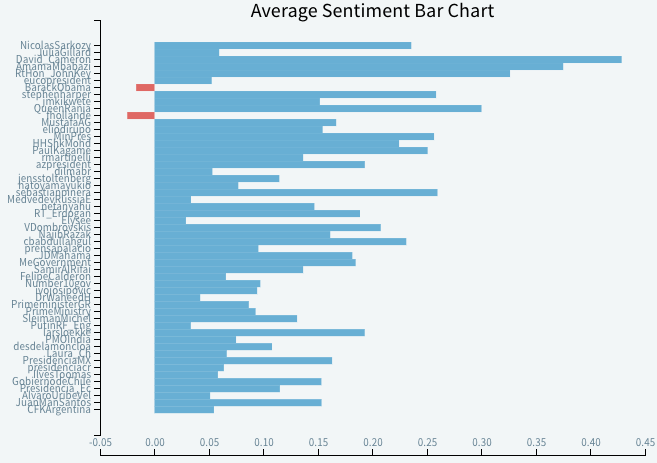
\includegraphics[height=7cm,width=\columnwidth, keepaspectratio]{imgs/all-pos.png}
 \caption{Average sentiment bar chart showing an overwhelmingly majority of positive sentiment tweets. All but two for all of the users that posted tweeted something happy showing that as a group World Leaders try to show positive attitudes to the public.. }
 \label{fig:all-pos}
\end{figure}

\begin{figure}[tb]
 \centering % avoid the use of \begin{center}...\end{center} and use \centering instead (more compact)
 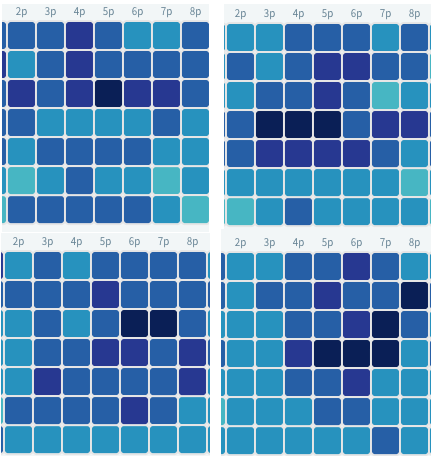
\includegraphics[height=7cm,width=\columnwidth, keepaspectratio]{imgs/heatmap-dense.png}
 \caption{Average sentiment bar chart showing an overwhelmingly majority of positive sentiment tweets. All but two for all of the users that posted tweeted something happy showing that as a group World Leaders try to show positive attitudes to the public.. }
 \label{fig:hmap-dense}
\end{figure}


\section{Conclusions}
%Give a summary of the problem and how your visualization has addressed it.

With the plethora of visualizations already available making use of Twitter data the goal of this visualization dashboard was to see how we can use visualizations to show shared similarities between users in a Twitter List.
The list was taken from the World Leaders list on Twitter \cite{twit-worldlist} and had to be heavily cleaned and translated to make all users eligible to be a part of the visualization.
The visualization consisted of four major visualizations including: tweet times heatmap, positive/negative average sentiment bar chart, tweet counts bar chart for a given month, and a bubble chart selecting the top 250 terms and the number users who used that word.

These visualizations showed that from merged Twitter data it is possible to use these visualization to pick out meaningful overlap in data to represent similarities between users.
The static tweet count bar chart showed that a majority of tweets currently occur closer to the present date.
Tweet time heatmaps showed there are specific time ranges that most world leaders tweet at.
The sentiment bar chart showed that for each month world leaders had an overall overwhelming positive attitude on these platforms.

In future work I believe there could many improvements in the user interactions for this dashboard.
One of them, namely filtering, would be an excellent feature in which user selection or user search for a word could affect multiple graphs and filter down the data.
This way the data wouldn't need to depend on a group to show individual values.
I believe in the future to help show the difference users in lists I could find other meaningful lists to compare the values retrieved in the project to the values retrieved from another group.
Its very possible that there are specific tweet times for other groups or the sentiment values may line up very similarly to what the world leaders got on average. 

\section*{Final Thoughts}
%This is an unnumbered section.
%Describe your experience working on the project. What were problems you faced? What things did you learn?

When approaching this project I had a clear mind of what I wanted to do and how I wanted to accomplish it.
I quickly realized that getting the desired result isn't always possible for some data.
One of the hardest learn lessons is that there are many great tools in visualization software, but more than half the battle in visualization goes into cleaning, preparing, and separating data in the desired format to get a great visualization.
Over the course of doing this project I've learned many data cleaning visualization techniques that I didn't expect that I would receive.
It has proven to be a valuable experience that will carry on into my future and enhance my Github portfolio nicely.

\bibliographystyle{abbrv-doi}
\bibliography{paper-template}
\end{document}

